\documentclass{article}
\usepackage{comment}
\usepackage[margin=1in]{geometry}%设置边距,符合Word设定
\usepackage{ctex} % 中文支持
\usepackage{enumitem}
\usepackage{amsmath,amssymb}    % 若你已加载过这类数学宏包,可忽略
\usepackage{tikz}
\usetikzlibrary{shapes.geometric, arrows, calc, positioning}
\usepackage{graphicx}
\usepackage{subcaption}
\usepackage{diagbox}
\usepackage{array}
\usepackage{listings}
\usepackage{tkz-euclide}

\usepackage{float} % 导入float宏包
\usepackage[ruled,vlined]{algorithm2e}
\title{光子输运问题模拟}
\author{耿滇沅\ \ \ \ \ \ 2021010237\ \ \ \ \ \ 核12}
\date{}
\begin{document}
\maketitle
%H强制图片位置跟随文本
\section{物理模型}
有一NaI(Tl)闪烁体尺寸$ \Phi 4\times 4cm$,即半径 $R=2cm$、高$ H=4cm$
(选做:闪烁体外部包裹 $0.2cm$ 厚的铝)。$^{137}Cs$ 点源在闪烁体中轴线上,与闪烁体顶面距离
$D=20cm$,粒子垂直向下入射进入晶体。
\begin{center}
    \begin{tikzpicture}
        % 定义颜色(可根据需要修改)
        \definecolor{paleYellow}{RGB}{255,255,204} % 淡黄
        \definecolor{paleBlue}{RGB}{204,229,255}   % 淡蓝
    
        % 外层圆柱填充(淡蓝色)
        % 利用底部和顶部的正面半椭圆弧以及垂直线段构成封闭路径
        \path[fill=paleBlue, draw=none]
            (-1.2,0) arc[start angle=180,end angle=0, x radius=1.2cm, y radius=0.7cm] 
            -- (1.2,3) arc[start angle=0,end angle=180, x radius=1.2cm, y radius=0.7cm]
            -- cycle;
    
        % 内层圆柱填充(淡黄色)
        \path[fill=paleYellow, draw=none]
            (-1,0) arc[start angle=180,end angle=0, x radius=1cm, y radius=0.5cm] 
            -- (1,3) arc[start angle=0,end angle=180, x radius=1cm, y radius=0.5cm]
            -- cycle;
    
        % 外层圆柱轮廓线
        \draw (0,0) ellipse (1.2cm and 0.7cm)[fill=paleBlue]; % 底部椭圆
        \draw (0,3) ellipse (1.2cm and 0.7cm)[fill=paleBlue]; % 顶部椭圆
        \draw (1.2,0) -- (1.2,3);
        \draw (-1.2,0) -- (-1.2,3);
    
        % 内层圆柱轮廓线
        \draw [dashed](0,0) ellipse (1cm and 0.5cm)[fill=paleYellow];   % 底部椭圆
        \draw (0,3) ellipse (1cm and 0.5cm)[fill=paleYellow];   % 顶部椭圆
        \draw (1,0) -- (1,3);
        \draw (-1,0) -- (-1,3);
        
        
        % 其余标注与辅助线
        \node at (0,5.3) {$^{137}Cs\ \gamma$源};
        \filldraw[red] (0,5) circle (2pt);
        \draw[->] (0.8,2.3) -- (1.5,2.3) node[right] {NaI(Tl)};
        \draw[->] (1.1,0.5) -- (1.5,0.5) node[right] {Al};
        \draw[<->] (-2,0) -- (-2,3) node[left,midway] {$H=4cm$};
        \draw[dashed] (-2,0) -- (0,0);
        \draw[dashed] (-2,3) -- (-0.5,3);
        \draw[dashed] (0,0) -- (0,5);
        \draw[<->] (0, 1.5) -- (1,1.5) ;
        \node at (2.1,1.5) {$R=2cm$};
        \draw[<->] (1, 3) -- (1.2,3) node[right] {$\delta=0.2cm$};
        \draw[->] (0,0) -- (1.8,0) node[right] {Y};
        \draw[->] (0,0) -- (0,4.5) node[right] {Z};
        \draw[->] (0,0) -- (-1.3,-1.1) node[right] {X};
        \filldraw[black] (0,0) circle (2pt);
    \end{tikzpicture}
\end{center}

用直接模拟法模拟光子在 NaI(Tl)闪烁体内的输运,简单地模拟低能光子在晶
体内的输运以及产生的能量沉积,忽略次级光子和电子的产生情况。在模拟过程中,假定粒子在两次碰撞之间按直线运动 ,且粒子之间的相互作用可以忽略。记录单个光子在闪烁体内损失的能量,
如果发生了光电效应,则认为损失了全部能量,如果是康普顿散射,沉积能量为碰撞前后的能量差,最后获得光子的总沉积能量。


理论上,在NaI(Tl)晶体外加上一层铝会降低康普顿坪的高度(至于降低幅度取决于铝层厚度以及康普顿效应反应截面的大小),
使得光子在探测器中沉积全部能量的概率增大。模拟粒子数相同时,表现在能谱结果上就是有铝层的能谱中全能峰计数要大于无铝层的能谱中全能峰计数。
事实上在模拟粒子数相同时,减小探测器的几何尺寸也会达到相应的效果。

\section{模拟思路}
为描述粒子在介质中的运动的状态,引入状态参数,它通常包括:粒子的空间位置
$\boldsymbol{r}$, 能量$E$ 和运动方向$ \boldsymbol{\varOmega} $,以 $\boldsymbol{S}^T=(\boldsymbol{r},E,\boldsymbol{\varOmega} )$ 表示。
有时还需要其他的参数,如粒子的 时间 $t$ 和附带的权重$W$ ,这时状态参数 为 $\boldsymbol{S}^{'T}=( \boldsymbol{r} , E , \boldsymbol{\varOmega}   ,t , W )$。
一个由源发出的粒子,在介质中经过 m 次碰撞
后的的状态参数为$\boldsymbol{S}^T_m=(\boldsymbol{r}_m,E_m,\boldsymbol{\varOmega}_m )$或 $\boldsymbol{S}^{'T}_m=( \boldsymbol{r}_m , E_m , \boldsymbol{\varOmega} _m  ,t _m, W_m )$
于是模拟一个粒子的运动过程,可以变成确定状态序列的问题:
\begin{equation}
    \begin{pmatrix}
        \boldsymbol{S}^{'}_0 & \boldsymbol{S}^{'}_1 & \cdots & \boldsymbol{S}^{'}_{M - 1} & \boldsymbol{S}^{'}_M 
    \end{pmatrix}
    =
    \begin{pmatrix}
    \boldsymbol{r}_0 & \boldsymbol{r}_1 & \cdots & \boldsymbol{r}_{M - 1} & \boldsymbol{r}_M \\
    E_0 & E_1 & \cdots & E_{M - 1} & E_M \\
    \boldsymbol{\varOmega} _0 & \boldsymbol{\varOmega} _1 & \cdots & \boldsymbol{\varOmega} _{M - 1} & \boldsymbol{\varOmega} _M\\
    t_0 & t_1 & \cdots & t_{M - 1} & t_M \\
    W_0 & W_1 & \cdots & W_{M - 1} & W_M \\ 
    \end{pmatrix}
\end{equation}


整个蒙卡模拟过程为:
\begin{enumerate}[label=\Alph*.]
    \item 确定粒子的初始状态$\boldsymbol{S}_0$:
    
    实际上就是要从粒子源的空间位置、能量和方向分布中抽样。

    设源分布为
    $f(\boldsymbol{r}_0,E_0,\boldsymbol{\varOmega }_0)=f_1(\boldsymbol{r}_0)f_2(E_0)f_3(\boldsymbol{\varOmega }_0)$
    则分别从各自的分布中抽样确定初始状态。
    
    特别的,对本例中的单向源:$\boldsymbol{r}_0=(0,0,H)\quad\boldsymbol{\varOmega }_0=(0,0,-1)$。
    \item 确定下一个碰撞点:
    
    已知状态$\boldsymbol{S}_{m-1}$,要确定状态$\boldsymbol{S}_m$,首先要确定下一个碰撞点的位置$\boldsymbol{r}_m$。


    从$f(L)$中抽样确定$L$,从指数分
    布$f(\rho )=e^{-\rho }\quad \rho \geq  0$抽样确定自由程数$\rho =\ln\xi $并解方程:

    对于单一介质
    \begin{equation}
        L=\frac\rho{\Sigma_t(E_{m-1})}=\frac{-\ln\xi}{\Sigma_t(E_{m-1})}
    \end{equation}

    对于多层介质,判断其可能范围
    $\sum_{i=1}^{l-1}\Delta L_i\cdot\Sigma_{t,i}(E_m)\leq\rho<\sum_{i=1}^l\Delta L_i\cdot\Sigma_{t,i}(E_m)$,得到:

    \begin{equation}
        L=\sum_{i=1}^{l-1}\Delta L_i+\frac{\rho-\sum_{i=1}^{l-1}\Delta L_i\cdot\Sigma_{t,i}(E_m)}{\Sigma_{t,L}(E_m)}=\sum_{i=1}^{l-1}\Delta L_i+\frac{-\ln\xi -\sum_{i=1}^{l-1}\Delta L_i\cdot\Sigma_{t,i}(E_m)}{\Sigma_{t,L}(E_m)}
    \end{equation}

    $L$确定后,则下一个碰撞点的位置:
    \begin{equation}
        \begin{gathered}
            \boldsymbol{r}_m=\boldsymbol{r}_{m-1}+L\cdot\boldsymbol{\varOmega}_{m-1}\\
            x_{m}=x_{m-1}+L\cdot u_{m-1}\\
            y_{m}=y_{m-1}+L\cdot v_{m-1}\\
            z_m=z_{m-1}+L\cdot w_{m-1}
        \end{gathered}
    \end{equation}

    如果$z_m\leq0$、或$z_m\geq H$、或$x_m^2+y_m^2\geq R^2$,则光子飞出晶体,光子历史终止。
    \item 确定被碰撞的原子核 :
    
    设介质由A、B、C 三种原子核组成,则介质的宏观总截面为:
    \begin{equation}
        \Sigma_t(E_{m-1})=\Sigma_t^A(E_{m-1})+\Sigma_t^B(E_{m-1})+\Sigma_t^C(E_{m-1})
    \end{equation}

    粒子与A、B、C 核发生碰撞的几率分别为:
    \begin{equation}
        P_A=\frac{\Sigma_t^A(E_{m-1})}{\Sigma_t(E_{m-1})}\quad P_B=\frac{\Sigma_t^B(E_{m-1})}{\Sigma_t(E_{m-1})}\quad P_C=\frac{\Sigma_t^C(E_{m-1})}{\Sigma_t(E_{m-1})}
    \end{equation}

    利用离散型随机变量的抽样方法,抽取随机数$\xi $,确定碰撞核种类:
    \begin{equation}
        \text{碰撞核种类} = \begin{cases}
            \text{A核} & \xi  \leq P_A \\
            \text{B核} & P_A< \xi  \leq P_A+P_B\\
            \text{C核} & \xi  > P_A+P_B
        \end{cases}
    \end{equation}
    \item 确定碰撞类型(两种方法) ,在大样本下,权重机制与随机抽样应该产生等效的统计结果:
    
    确定了碰撞的核(如B核)后,就要进一步确定碰撞类型。
    
    只考虑光电效应和康普顿效应,它们的微观截面分别为$\sigma_{pe}^B(E_{m-1})$、$\sigma_c^B(E_{m-1})$,其中:
    \begin{equation}
        \begin{gathered}
            \sigma_t^B(E_{m-1})=\sigma_{pe}^B(E_{m-1})+\sigma_c^B(E_{m-1})\\
            P_{pe}=\frac{\sigma_{pe}^B(E_{m-1})}{\sigma_t^B(E_{m-1})}\\
            P_c=\frac{\sigma_{c}^B(E_{m-1})}{\sigma_t^B(E_{m-1})}
        \end{gathered}
    \end{equation}

    \item (深穿透或大系统问题)光子进入探测器前会经历多次散射,采用权重机制:
    
    \begin{equation}
        \begin{gathered}
            \text{对源光子:}W_0=1\\
            \text{散射权重:}W_m=W_{m-1}\frac{\Sigma_c^B(E_{m-1})}{\Sigma_t^B(E_{m-1})}=W_{m-1}\cdot P_c^B\\
        \end{gathered}
    \end{equation}
    
    将粒子到达探测器前的随机事件分解成两个固定的“确定性事件”,即吸收和散射。
    
    只有散射才可能进入探测器,而吸收则一定终止光子历史,散射后将以权重$W_{in}$进入探测器。

    进入探测器后就不能用加权法了,只能用直接模拟法。

    粒子权重$W<10^{-4}$时,采用俄国轮盘赌的方法,令$0 < q < 1\quad W_q = W / q$,取随机数$\xi $:
    \begin{equation}
        \begin{gathered}
            W = q \cdot W_q + (1 - q) \cdot 0 \\
            P(W = W_q) = q \\
            P(W = 0) = 1 - q \\
            W=
        \begin{cases}
            W_q&\xi\leq q\text{继续跟踪}\\
            0&\xi> q\text{停止跟踪}
        \end{cases}
        \end{gathered}
    \end{equation}

    通过边界条件、能量阈值以及光子权重$W$是否为零,判断光子历史是否终止。

    \item 直接模拟法分析光子在探测器中的作用:
    
    抽取随机数$\xi $,确定反应类型
    
    \begin{equation}
        \text{反应类型} = \begin{cases}
            \text{光电效应:吸收全部能量光子的历史终止} & \xi  \leq P_{pe} \\
            \text{康普顿效应:进一步
            确定康普顿散射后光子的能量和方向} &  \xi  > P_{pe}
        \end{cases}
    \end{equation}

    通过边界条件、能量阈值等,判断光子历史是否终止。

    
    
    \item 确定康普顿散射后光子的能量和方向:
    
    光子发生康普顿散射后,其能量分布密度函数为:
    \begin{equation}
        \begin{gathered}
            f(\frac x{\alpha})=\frac1{K(\alpha)}\left[\left(\frac{\alpha+1-x}{\alpha\cdot x}\right)^2+\frac1x-\frac1{x^2}+\frac1{x^3}\right]\quad1\leq x\leq1+2\alpha \\
            K(\alpha)=\left[1-\frac{2(\alpha+1)}{\alpha^2}\right]\ln(1+2\alpha)+\frac12+\frac4\alpha-\frac1{2(1+2\alpha)^2}\\
            x= \frac{\alpha}  {\alpha ^{\prime }}\quad \alpha = E/ m_0c^2\quad \alpha ^{\prime }= E^{\prime }/ m_0c^2
        \end{gathered}
    \end{equation}

    $\alpha$和$\alpha^\prime$分别为光子散射前后的能量,以$m_0c^2$ 为单位,$m_0$为电子静止质量,$c$为光速。

    光子康普顿散射能量分布的抽样方法为:
    \begin{figure}[H]
        \centering
        \begin{tikzpicture}[node distance=3.2cm, scale=0.7, transform shape]
            \tikzset{
                > = stealth,
                block/.style = {rectangle, rounded corners, draw=black, fill=white,
                                text width=8em, align=center, minimum height=2em},
                decision/.style = {diamond, draw=black, fill=white, aspect=1.5,
                                    text width=8em, align=center, inner sep=0pt},
                line/.style = {->, thick}
            }
    
            % 开始节点
            \node [block, text width=12em] (start) {生成 $\xi_1,\ \xi_2,\ \xi_3 \in (0,1)$};
    
            % 判断1
            \node [decision, below of=start, text width=8em] (dec1) {$\xi_1 \le \frac{27}{4\alpha+29}$?};
    
            % 左分支
            \node [block, below left=1cm and 1.5cm of dec1] (x1def) {$x_1 = \frac{1 + 2\alpha}{1 + 2\alpha \xi_2}$};
            \node [decision, below of=x1def, text width=9em] (dec2) {$\xi_3 \le \frac{1}{2}\biggl[\biggl(\frac{\alpha+1 - x_1}{\alpha}\biggr)^2 + 1\biggr]$?};
    
            % 右分支
            \node [block, below right=1cm and 1.5cm of dec1] (x2def) {$x_2 = 1 + 2\alpha \xi_2$};
            \node [decision, below of=x2def, text width=9em] (dec3) {$\xi_3 \le \frac{27(x_2 - 1)^2}{4 x_2^3}$?};
    
            % 结果节点
            \node [block, below of=dec2] (xeqx1) {$x = x_1$};
            \node [block, below of=dec3] (xeqx2) {$x = x_2$};
    
            % 路径连接
            \draw [line] (start) -- (dec1);
    
            % dec1判断
            \draw [line] (dec1) -| node[anchor=south, above left]{是}(x1def);
            \draw [line] (dec1) -| node[anchor=south, above right]{否}(x2def);
    
            % 左分支逻辑
            \draw [line] (x1def) -- (dec2);
            \draw [line] (dec2) -- node[anchor=west]{是}(xeqx1);
    
            % 从dec2否分支返回顶部start
            \draw [line] (dec2.west)   |- node[anchor=south, above left]{否}(start.west);
    
            % 右分支逻辑
            \draw [line] (x2def) -- (dec3);
            \draw [line] (dec3) -- node[anchor=west]{是}(xeqx2);
    
            % 从dec3否分支返回顶部start
            \draw [line] (dec3.east)  |- node[anchor=south, above right]{否}(start.east);
    
        \end{tikzpicture}
    
        \caption{流程图示意}
    \end{figure}
        
    $x $的抽样确定后,散射后的能量为:
    \begin{equation}
        E_{m+1}=\alpha^{\prime}\cdot m_0c^2=\frac{\alpha}{x}\cdot m_0c^2=\frac{E_m}{x}
    \end{equation}

    光子的康普顿散射角余弦$\mu _L=\cos\theta _L$与其散射前后的能量有关,其分布密度函数为:
    \begin{equation}
        \begin{gathered}
            f(\mu_L)=\delta(1-\frac1{\alpha^{\prime}}+\frac1\alpha-\mu_L)\\
            \text{抽样方法为:}\mu_L=1-\frac1{\alpha^{\prime}}+\frac1\alpha 
        \end{gathered}
    \end{equation}

    $\theta _L$确定后,还需要确定方位角并最终确定散射后光子的运动方向:
    \begin{figure}[H]
        \centering
        \includegraphics[width=0.3\textwidth]{jiaodu.png}
        \label{}
    \end{figure}
    
    一般地,$\varOmega ^T_m=(u_m,v_m,w_m)$与$\varOmega ^T_{m-1}=(u_{m-1},v_{m-1},w_{m-1})$的变换关系为:
    \begin{equation}
        \begin{gathered}
            u_m=\frac{-bcw_{m-1}u_{m-1}+bdv_{m-1}}{\sqrt{u_{m-1}^2+v_{m-1}^2}}+au_{m-1}\\
            v_{m}=\frac{-bcw_{m-1}v_{m-1}-bdu_{m-1}}{\sqrt{u_{m-1}^2+v_{m-1}^2}}+av_{m-1}\\
            w_m=bc\sqrt{u_{m-1}^2+v_{m-1}^2}+aw_{m-1}\\
            a=\cos\theta_L\quad b=\sin\theta_L=\sqrt{1-a^2}\quad c=\cos\varphi\quad d=\sin\varphi\\
            \text{方位角}\varphi\text{在 }[0,2\pi]\text{ 上均匀分布}
        \end{gathered}
    \end{equation}

    特别地,$u_{m-1}^2+v_{m-1}^2\to0$时:
    \begin{equation}
        \begin{aligned}u_m&=bc\\v_m&=bd\\w_m&=aw_{m-1}\end{aligned}
    \end{equation}
    \item 记录结果,重复以上过程直至出现粒子从系统逃脱或经碰撞被吸收,光子的随机游动终止:

    记录光子在探测器中发生的每次碰撞所损失的能量$E(D)=\Sigma E(D)_m$,对第m次碰撞的粒子:
    \begin{equation}
        E_D(m)=
        \begin{cases}
            E_{m-1}-E_m&\text{康普顿效应}\\
            E_{m-1}&\text{光电效应}
        \end{cases}
    \end{equation}

    共跟踪了N个光子,计算NaI(Tl)晶体探测效率:
    \begin{equation}
        \begin{gathered}
            \text{记录到的光子数:}N_c=\sum_{n=1}^N\eta_n\\
            \text{探测效率的近似值:}\hat{\eta}_N=\frac{N_c}{N}=\frac{1}{N}\sum_{n=1}^N\eta_n
        \end{gathered}
    \end{equation}

    为了得到光子能量沉积谱,事先将能量分成若干个等距间隔:
    \begin{equation}
        E_{min}=E_0<E_1<\cdots<E_I=E_{max}
    \end{equation}


    光子以权重$W_{in}$进入探测器并沉积能量$E_D$,落在第$i$个能量间隔$\Delta E_i$,其能量计数器中加$W_{in}$。
\end{enumerate}



考虑到测量系统的分辨率,实际记录的能量为沉积能量的高斯展宽,且在能量$E$处的半高
宽:
\begin{equation}
    FWHM(E)=0.01+0.05\sqrt{E+0.4E^2}
\end{equation}
其中能量$E$的单位为 MeV

记录能量为:
\begin{equation}
    \begin{gathered}
    E^{\prime }= E+ \sigma \cdot x\\
    \sigma = FWHM/ 2\sqrt {2\ln 2}\approx 0. 4247\cdot FWHM 
    \end{gathered}
\end{equation}
$x$为服从标准正态分布的随机变量。


\begin{figure}[H]
    \centering
    \includegraphics[width=0.45\textwidth]{chengxuliucheng.png}
    \caption{蒙特卡罗程序结构}
    \label{}
\end{figure}

\begin{comment}
\begin{algorithm}[H]
    \caption{光子输运的蒙特卡罗模拟}
    \KwIn{光子数 $N$,源能量 $E_0$,几何参数 $R$, $H$,材料数据}
    \KwOut{探测效率,峰总比,能量分辨率,能谱图}
    
    \textbf{初始化:} 加载材料的截面数据\;
    定义分辨率函数 \texttt{apply\_resolution}\;
    定义截面插值函数 \texttt{interpolate\_cross\_sections}\;
    定义反应类型确定函数 \texttt{determine\_reaction\_type}\;
    定义自由程计算函数 \texttt{L\_calculate}\;
    
    \For{$i = 1$ \textbf{到} $N$}{
        初始化光子的位置和方向\;
        初始化光子能量为 $E_0$\;
    
        \While{光子在探测器内}{
            计算自由程并移动光子\;
            确定反应类型(光电效应或康普顿效应)\;
            更新沉积能量和光子状态\;
    
            \If{光子能量低于阈值}{
                对沉积能量应用高斯展宽\;
                将能量记录到能谱的对应区间\;
                退出循环\;
            }
        }
        \If{光子被探测到}{
            增加探测光子计数\;
            \If{能量在全能峰范围内}{
                增加全能峰计数\;
            }
        }
    }
    
    计算探测效率和峰总比\;
    估算 $E_0$ 处的能量分辨率\;
    绘制能谱图并分析\;
    
\end{algorithm}
\end{comment}



\section{$ N_{\gamma }=10^6$模拟结果分析}

\begin{figure}[H]
    \centering
    \begin{subfigure}[b]{0.3\textwidth}
        \centering
        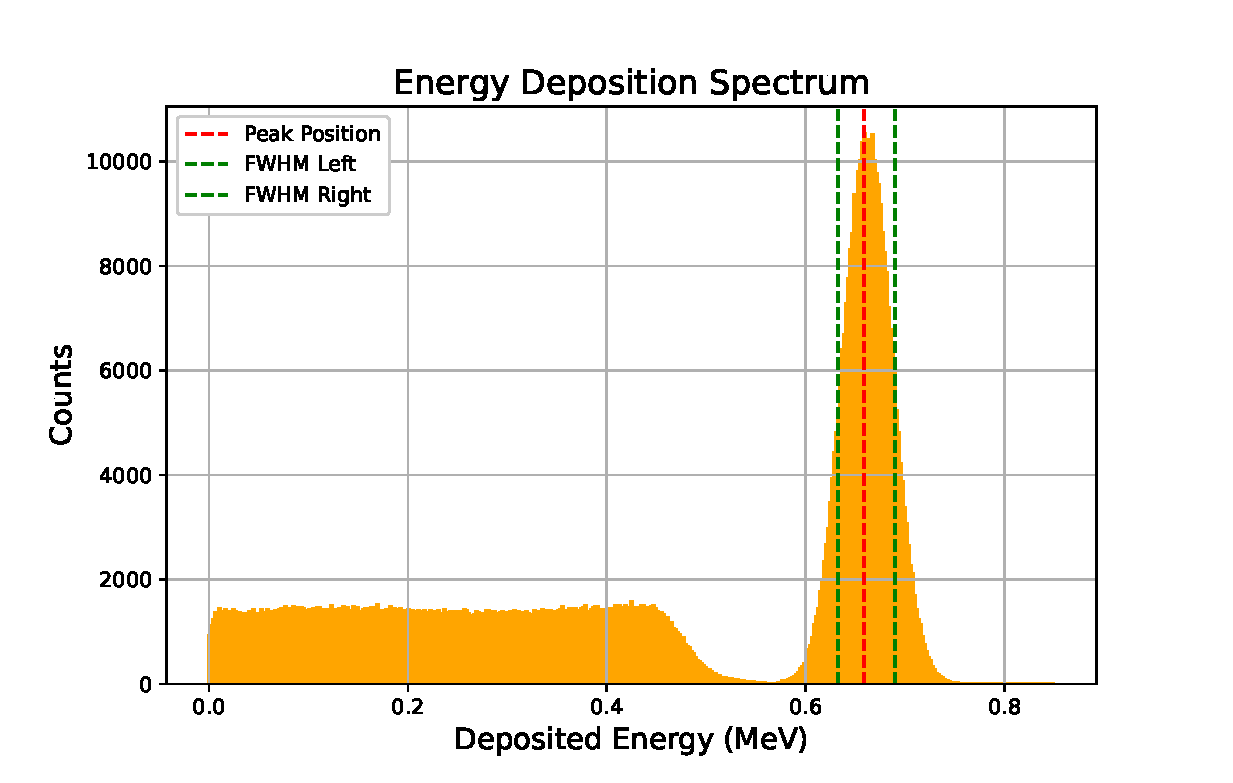
\includegraphics[width=\textwidth]{000.eps}
        \caption{$\delta _{Al}=0cm\quad R=1cm$}
        \label{small_R}
    \end{subfigure}
    \hfill
    \begin{subfigure}[b]{0.3\textwidth}
        \centering
        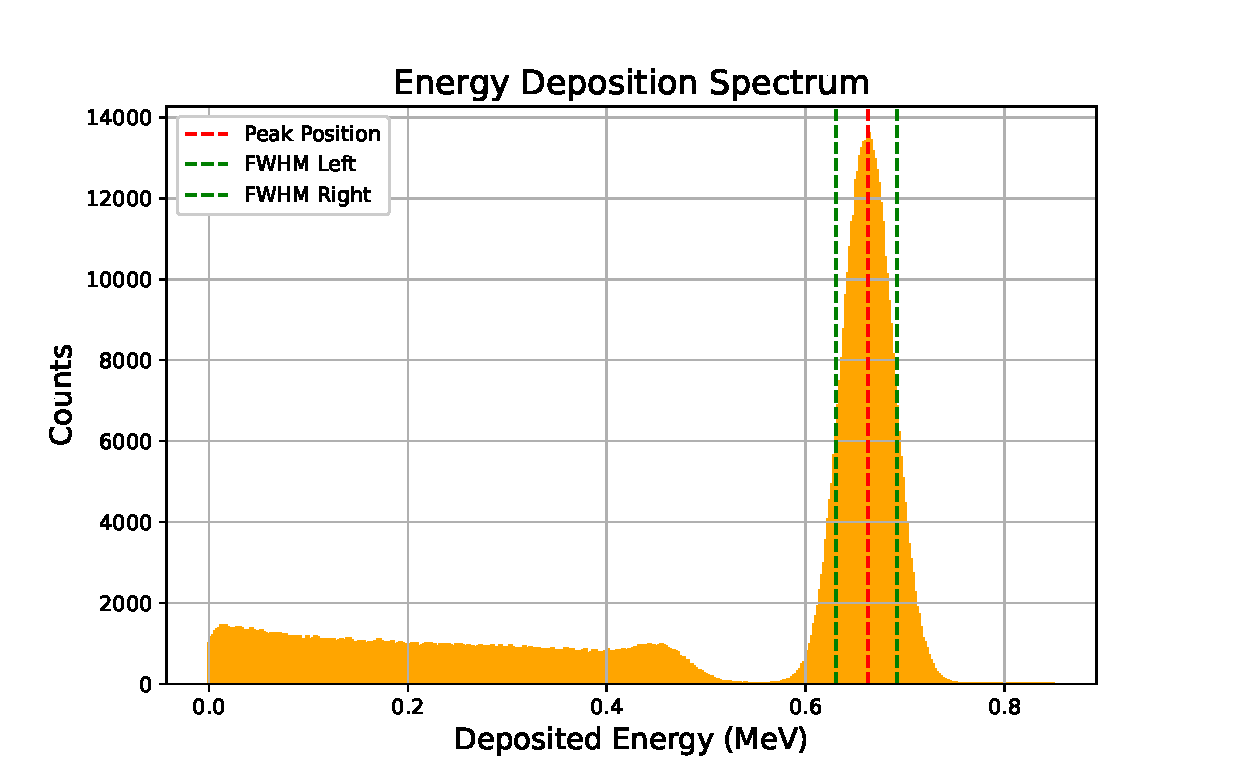
\includegraphics[width=\textwidth]{001.eps}
        \caption{$\delta _{Al}=0cm\quad R=2cm$}
        \label{no_Al}
    \end{subfigure}
    \hfill
    \begin{subfigure}[b]{0.3\textwidth}
        \centering
        \includegraphics[width=\textwidth]{002.eps}
        \caption{$\delta _{Al}=0.2cm\quad R=2cm$}
        \label{Al}
    \end{subfigure}
    \caption{不同几何尺寸以及Al厚度下的能谱图对比}
\end{figure}

\begin{table}[h]
    \centering
    \caption{不同几何尺寸以及Al厚度下的能谱数据对比}
    \begin{tabular}{ccccccc}
        \hline
        变参量/cm & $N_m$ & $N_p$ & 探测效率 & 峰总比 & 峰位、半高宽$MeV$ &能量分辨率 \\
        \hline
        $\delta _{Al}=0\quad R=1$ & 665098 & 324469 & 66.51\% & 48.78\% & 0.659、0.058 &8.8\%  \\

        $\delta _{Al}=0\quad R=2$ & 664773 & 420200 & 66.48\% & 63.21\% & 0.663、0.062 &9.35\%  \\
        
        $\delta _{Al}=0.2\quad R=2$ & 664156 & 470718 & 66.42\% & 70.88\% & 0.665、0.06 &9.023\%  \\
        
        \hline
    \end{tabular}
    \label{3case1}
\end{table}

显然增大NaI(Tl)探测器的几何尺寸或者在外围加上一层铝箔都可以降低康普顿坪的高度,因为这两种方法都能减小光子逃逸的概率。

图\ref{small_R}和图\ref{no_Al}显示了没有铝箔将NaI(Tl)探测器的几何尺寸为$R=1cm$、$R=2cm$时的蒙卡模拟能谱,
从表\ref{3case1}中能看到,随着NaI(Tl)探测器几何尺寸的增大,峰总比提高了约14.43\%,在$N_{\gamma }=10^6$时,在探测器内沉积全部能量的光子数目
增加了95731个,这是很可观的提升。相应的,在$0.662MeV$处的能量分辨率也提高了,从8.8\%提升到了9.35\%。

图\ref{no_Al}和图\ref{Al}显示了NaI(Tl)探测器的几何尺寸为$R=2cm$时,在探测器外围包裹铝箔前后的蒙卡模拟能谱,
从表\ref{3case1}中能看到,增加铝箔后,峰总比提高了约7.67\%,在$N_{\gamma }=10^6$时,在探测器内沉积全部能量的光子数目
增加了50518个,相较于没有铝箔时有明显的提升。
\begin{figure}[H]
    \centering
    \begin{subfigure}[b]{0.3\textwidth}
        \centering
        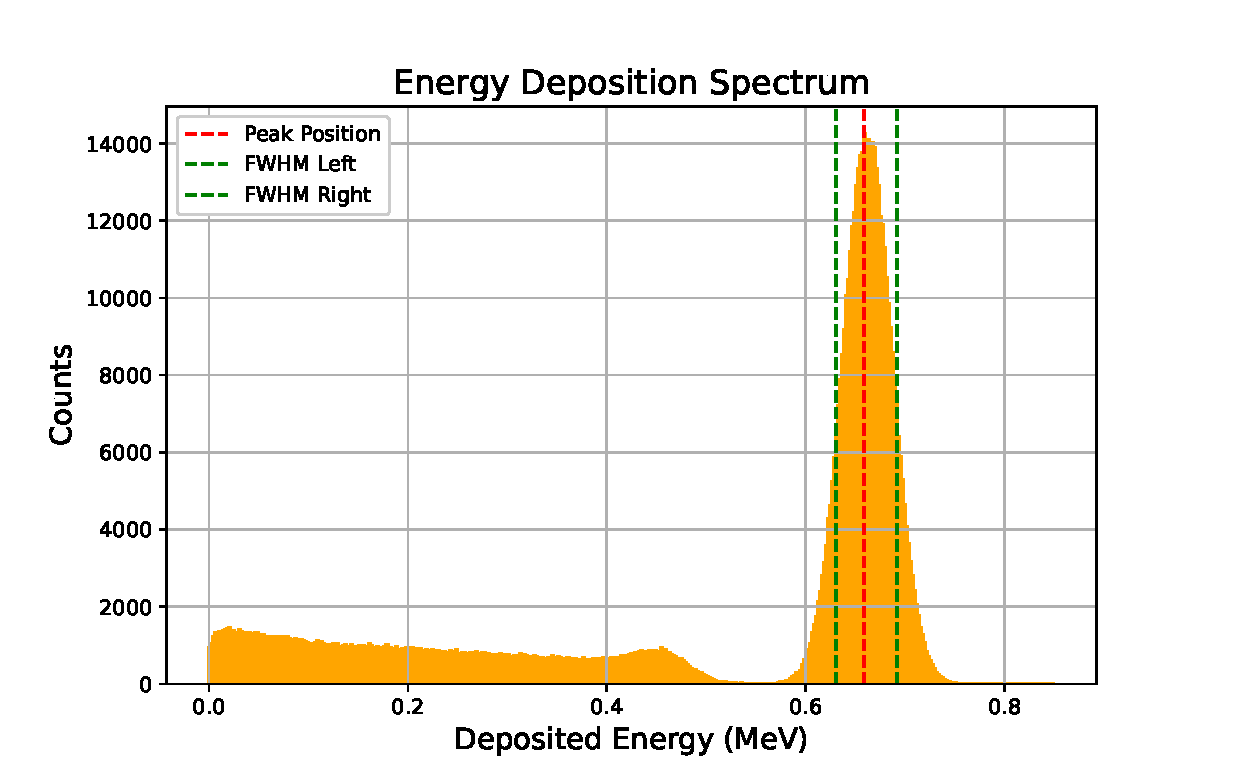
\includegraphics[width=\textwidth]{003.eps}
        \caption{$\delta _{Al}=0\quad R_{NaI}=2.4$}
        \label{R_no_Al}
    \end{subfigure}
    \hspace{5pt} % 调整间距(5pt 可根据需要修改)
    \begin{subfigure}[b]{0.3\textwidth}
        \centering
        \includegraphics[width=\textwidth]{004.eps}
        \caption{$\delta _{Al}=0.4\quad R_{NaI}=2$}
        \label{R_Al}
    \end{subfigure}
    \caption{相同几何尺寸不同Al厚度下的能谱图对比}
\end{figure}

\begin{table}[h]
    \centering
    \caption{相同几何尺寸不同Al厚度下的能谱数据对比}
    \begin{tabular}{ccccccc}
        \hline
        变参量/cm & $N_m$ & $N_p$ & 探测效率 & 峰总比 & 峰位、半高宽$MeV$ &能量分辨率 \\
        \hline
        $\delta _{Al}=0\quad R_{NaI}=2.4$ & 664758 & 440858 & 66.48\% & 66.32\% & 0.659、0.062 &9.41\%  \\

        $\delta _{Al}=0.4\quad R_{NaI}=2$ & 665217 & 475272 & 66.52\% & 71.45\% & 0.663、0.062 &9.35\%  \\
        
        \hline
    \end{tabular}
    \label{2case1}
\end{table}

图\ref{R_no_Al}和图\ref{R_Al}显示了在相同的探测器几何尺寸$R=2.4cm$,NaI(Tl)与铝箔不同尺寸占比下的蒙卡模拟能谱,
从表\ref{2case1}中能看到,将探测器材料全是NaI(Tl)($R_{NaI}=2.4cm\quad \delta _{Al}=0cm$)改为内层NaI(Tl)、外层铝箔($R_{NaI}=2cm\quad \delta _{Al}=0.4cm$)时,
峰总比提高了约5.18\%,在$N_{\gamma }=10^6$时,在探测器内沉积全部能量的光子数目
增加了34414个,相较于探测器材料全是NaI(Tl)时有一定的提升。
在考虑材料成本的情况下,选择更经济的铝箔作为外层材料,不仅能够有效降低成本,还能够在一定程度上提高峰总比和能量分辨率,从而实现性能与成本的双重优化。

图\ref{Al}和图\ref{R_Al}显示了在相同的NaI(Tl)几何尺寸$R=2cm$,不同铝箔厚度下的蒙卡模拟能谱,
从表\ref{3case1}、\ref{2case1}中能看到,$R_{NaI}=2cm$时将$\delta _{Al}$从$0.2cm$增加到$0.4cm$时,
峰总比提高了约0.57\%,在$N_{\gamma }=10^6$时,在探测器内沉积全部能量的光子数目
增加了约4454个,前后变化不大。这就意味再增加铝箔厚度带来的提升有限,一般没有必要为了很小的增幅而花费更多材料。

探测效率的变化并不明显,这是由我们的蒙特卡洛模拟假设所决定的。在模拟中,我们将所有粒子的方向都设为:$\varOmega =(0,0,-1)$,光子与探测器仅发生光电效应和康普顿效应,一旦发生相互作用,光子就会在探测器内沉积能量。
所以光子只可能在第一次抽样决定自由程时不会在探测器里沉积能量,光子$0.662MeV$的能量对应$\Sigma_t=0.2721cm^{-1}$,不被探测到的概率计算如下:
\begin{equation}
    \begin{gathered}
        L=\frac{-\ln(\xi)}{\Sigma_t} =\frac{-\ln(\xi)}{0.2721} >4\\
        \xi<0.3368\\
        P_{detected}=1-\xi=66.32\%\quad P_{undetected}=33.68\%
    \end{gathered}
    \label{Pdetected}
\end{equation}

我们在整个模拟过程中并未改变探测器的高度,所以得到的探测效率应该在66.32\%附近,这与我们模拟得到的探测效率相符,模拟探测效率与实际探测效率之间的差别很大程度上取决于模拟粒子数,这是蒙卡模拟本身特性决定的。
探测效率之间的微小差别主要是由统计误差引起的。

想要验证式(\ref{Pdetected})的正确性,我们可以改变探测器的高度,观察探测效率的变化:
\begin{table}[h]
    \centering
    \caption{不同高度下的探测效率对比}
    \begin{tabular}{ccccccc}
        \hline
        $H/cm$& 2 & 4 & 6 & 8  \\
        \hline
        理论 & 41.97\% & 66.32\% & 80.46\% & 88.66\%   \\
        实际 & 42.10\% & 66.50\% & 80.66\% & 88.84\%   \\
        \hline
    \end{tabular}
\end{table}

在闪烁探测器设计中,NaI(Tl) 作为高效的闪烁体材料,能够将入射光子的能量高效地转化为大量的可见光信号,这对光子的高效探测至关重要。  
铝 作为金属材料,其主要优势在于良好的反射性能和 屏蔽作用。将铝用作外层,可以有效地反射 NaI(Tl) 闪烁体发出的光信号回到探测器内部,从而提升探测效率。但若将铝放在内层,它无法有效吸收光子能量,也不能生成光信号,反而会影响光信号的传输与输出,降低探测器的整体性能。  
综合考虑成本与性能的关系,合理选择NaI(Tl)的半径与铝箔的厚度,可以实现性能与成本的双重优化。


\section{误差估计}
通常,蒙特卡罗方法的误差ε定义为:
\begin{equation}
    \begin{gathered}
        \varepsilon = \frac{\lambda \alpha \sigma}{\sqrt{N}} \\
    \hat{\sigma}=\sqrt{\frac{1}{N}\sum_{i=1}^NX_i^2-\left(\frac{1}{N}\sum_{i=1}^NX_i\right)^2}
    \end{gathered}
    \label{error}
\end{equation}
用$\hat{\sigma}$代替$\sigma$

这里误差估计取置信水平 1$- \alpha = 0. 95$, $\lambda _{\mathrm{a} }\approx 2. 0$,$N_{\gamma }=10^6 \quad R_{NaI}=2cm\quad \delta _{Al}=0.2cm$模拟九次($N=9$)。

\begin{table}[H]
    \centering
    \caption{模拟9次的探测效率、峰总比}
    \begin{tabular}{cccccccccccc}
        \hline
        序号 & 1 & 2 & 3 & 4 & 5 & 6 & 7 & 8 & 9 \\
        \hline
        $\eta $ & 66.44\% & 66.54\% & 66.53\% & 66.46\% & 66.62\% & 66.53\% & 66.50\% & 66.59\% & 66.51\% \\
        
        $R $& 70.91\% & 70.76\% & 70.83\% & 70.92\% & 70.81\% & 70.81\% & 70.98\% & 70.88\% & 70.89\% \\
        \hline
    \end{tabular}
    \label{tab:example}
\end{table}

用公式\ref{error}计算得到,在95\%的置信水平下:
\begin{equation}
    \begin{gathered}
        \text{探测效率:}\eta  = 66.52\%\quad \varepsilon _{\eta }=\pm  0.05\%\\
        \text{峰总比:}R=70.87\%\quad \varepsilon _R=\pm 0.06\%\\
    \end{gathered}
    \label{error1}
\end{equation}


\end{document}

